\documentclass{article}
\usepackage{graphicx}
\usepackage[utf8]{inputenc}
\usepackage[T1]{fontenc}
\usepackage{fouriernc}
\usepackage[margin=1in]{geometry}
\usepackage{amsmath}
\begin{document}

\begin{titlepage}
	\centering 
	\scshape
	\vspace*{\baselineskip}
	\rule{\textwidth}{1.6pt}\vspace*{-\baselineskip}\vspace*{2pt}
	\rule{\textwidth}{0.4pt} 
	\vspace{0.75\baselineskip}
	
	{\Large CS 374 : Computational and Numerical Methods \\\vspace{0.75\baselineskip} Set 11}
	\vspace{0.75\baselineskip}
	
	\rule{\textwidth}{0.4pt}\vspace*{-\baselineskip}\vspace{3.2pt} 
	\rule{\textwidth}{1.6pt}
	
	\vspace{2\baselineskip}  
	 Solution of Non-linear Equation
	
	\vspace*{3\baselineskip}
	
	\vspace{0.5\baselineskip} %originally 0.5
	
	{\scshape\large Purvil Mehta (201701073) \\ Bhargey Mehta (201701074) \\} 
	
	\vspace{1\baselineskip} 
	
	\textit{Dhirubhai Ambani Institute of Information and Communication Technology \\ Gandhinagar\\} 
	\vspace*{2\baselineskip}
	\today


\end{titlepage}
\newpage
\section{Visulization}
\begin{figure}[!h]
    \centering
    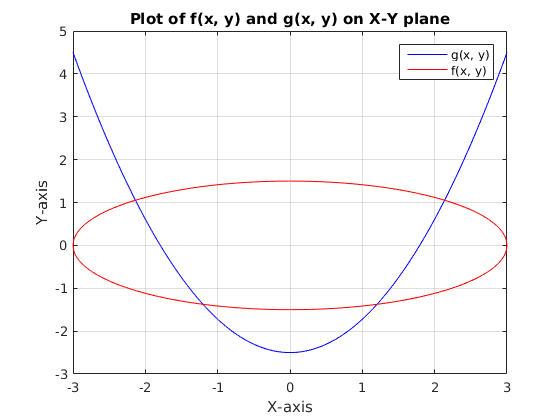
\includegraphics[scale = 0.8]{11_1.png}
\end{figure}

\section{Initial value = $[-1 , -1]$}
\begin{table}[!h]\centering{\Large
\begin{tabular}{|c|c|c|c|c|}
\hline
itrno & $x$ & $y$ \\
\hline
1& -1      & -1      \\
2&-1.1702 & -1.4574 \\
3&-1.2022 & -1.3768 \\
4&-1.2032 & -1.3741 \\
5&-1.2032 & -1.3741 \\
\hline
\end{tabular}}
\end{table}
\newpage

\section{Initial value = $[-1, 1]$}
\begin{table}[!h]\centering{\Large
\begin{tabular}{|c|c|c|c|c|}
\hline
itrno & $x$ & $y$ \\
\hline
1 & -1      & 1      \\
2 & -2.7846 & 1.0538 \\
3 & -2.2125 & 1.0527 \\
4 & -2.1385 & 1.0527 \\
5 & -2.1372 & 1.0527 \\
6 & -2.1372 & 1.0527 \\
\hline
\end{tabular}}
\end{table}

\section{Initial value = $[1, 1]$}
\begin{table}[!h]\centering{\Large
\begin{tabular}{|c|c|c|c|c|}
\hline
itrno & $x$ & $y$ \\
\hline
1 & 1      & 1      \\
2 & 2.7846 & 1.0538 \\
3 & 2.2125 & 1.0527 \\
4 & 2.1385 & 1.0527 \\
5 & 2.1372 & 1.0527 \\
6 & 2.1372 & 1.0527 \\
\hline
\end{tabular}}
\end{table}




\section{Initial value = $[1, -1]$}
\begin{table}[!h]\centering{\Large
\begin{tabular}{|c|c|c|c|c|}
\hline
itrno & $x$ & $y$ \\
\hline
1 & 1      & -1      \\
2 & 1.1702 & -1.4574 \\
3 & 1.2022 & -1.3768 \\
4 & 1.2032 & -1.3741 \\
5 & 1.2032 & -1.3741 \\
\hline
\end{tabular}}
\end{table}


\end{document}